\section{Zelda: Skyward Sword}

\begin{figure}[htbp]
\begin{center}
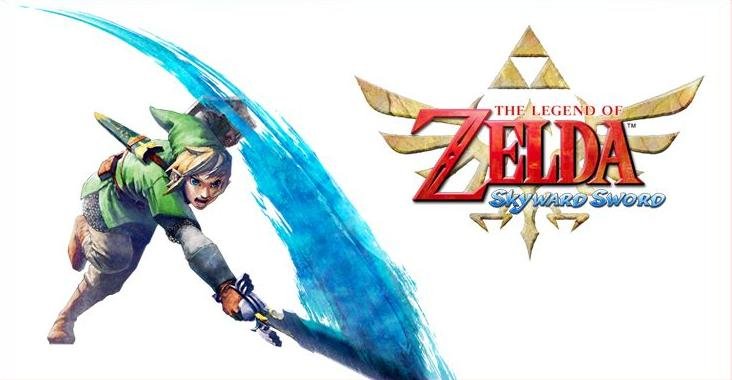
\includegraphics[width=.60\textwidth]{./imagenes/skyward.jpg}
\caption{Zelda: Skyward Sword}
\label{Zelda: Skyward Sword}
\end{center}
\end{figure}
Zelda: Skyward Sword\footnote{\url{http://zelda.com/skywardsword/}} es el primer Zelda en ofrecerte total control de la espada y escudo via wiimote + nunchuck. Fue publicado en Noviembre del 2011 y ha sido uno de los juegos de Zelda más controversiales por su único modo de jugarlo con controles de movimiento.

La premisa del juego es que eres un chico (Link) que vive en una comunidad en una isla flotante y debes emprender un viaje a la superficie (Hyrule) para rescatar a Zelda.

\subsubsection{¿Por qué es uno de mis juegos favoritos?}
\begin{itemize}
\item[Gianni Carlo] Las reglas del juego son similares a los anteriores juegos de Zelda con el agregado que ahora cada enemigo fue diseñado con los controles de moviemiento en mente, no basta con agitar de izquierda a derecha el control para poder pasar el juego, y esto ayuda en gran parte a sumergirte en el juego ya que debes atacar de cierta forma a los enemigos y/o repeler ataques con tu escudo en el momento preciso sino recibes una penalidad. A pesar de esto, el juego no es atractivo para todo el mundo debido a la única opción de controles a los que alegan que no responden con suficiente precisión o a veces ni responden. Para mi, el gran interés del juego, aparte de presentar el origen de la historia del universo de Zelda, es el nuevo estilo de jugarlo y la experiencia de inmersión única que presenta a cualquier fan de la serie (los motion controls de Twilight Princess para Wii no cuentan en mi opinión ya que eran tan solo un test para ver que tan buena sería la acogida para implementarlo como única opción en el siguiente Zelda).
\end{itemize}